% !TeX root = ../../main.tex
\newpage
\section{Generator sztucznych danych}

Generator sztucznych danych został napisany w języku \textit{JavaScript} jako aplikacja internetowa, z prostym i czytelnym interfejsem użytkownika.
Do zbudowania interfejsu wykorzystano bibliotekę \textit{React}\footnote{https://reactjs.org/}.
Ekran aplikacji dzieli się na dwie częsci:
\begin{itemize}
  \item Instrukcja, objaśniająca jak obsługiwać generator za pomocą klawiatury i myszy
  \item Scena 3D, na której rysowany generowany jest obraz
\end{itemize}
Scena 3D rysowana jest za pomocą biblioteki \textit{Three.js}\footnote{https://threejs.org/}.

\begin{figure}[!htb]
  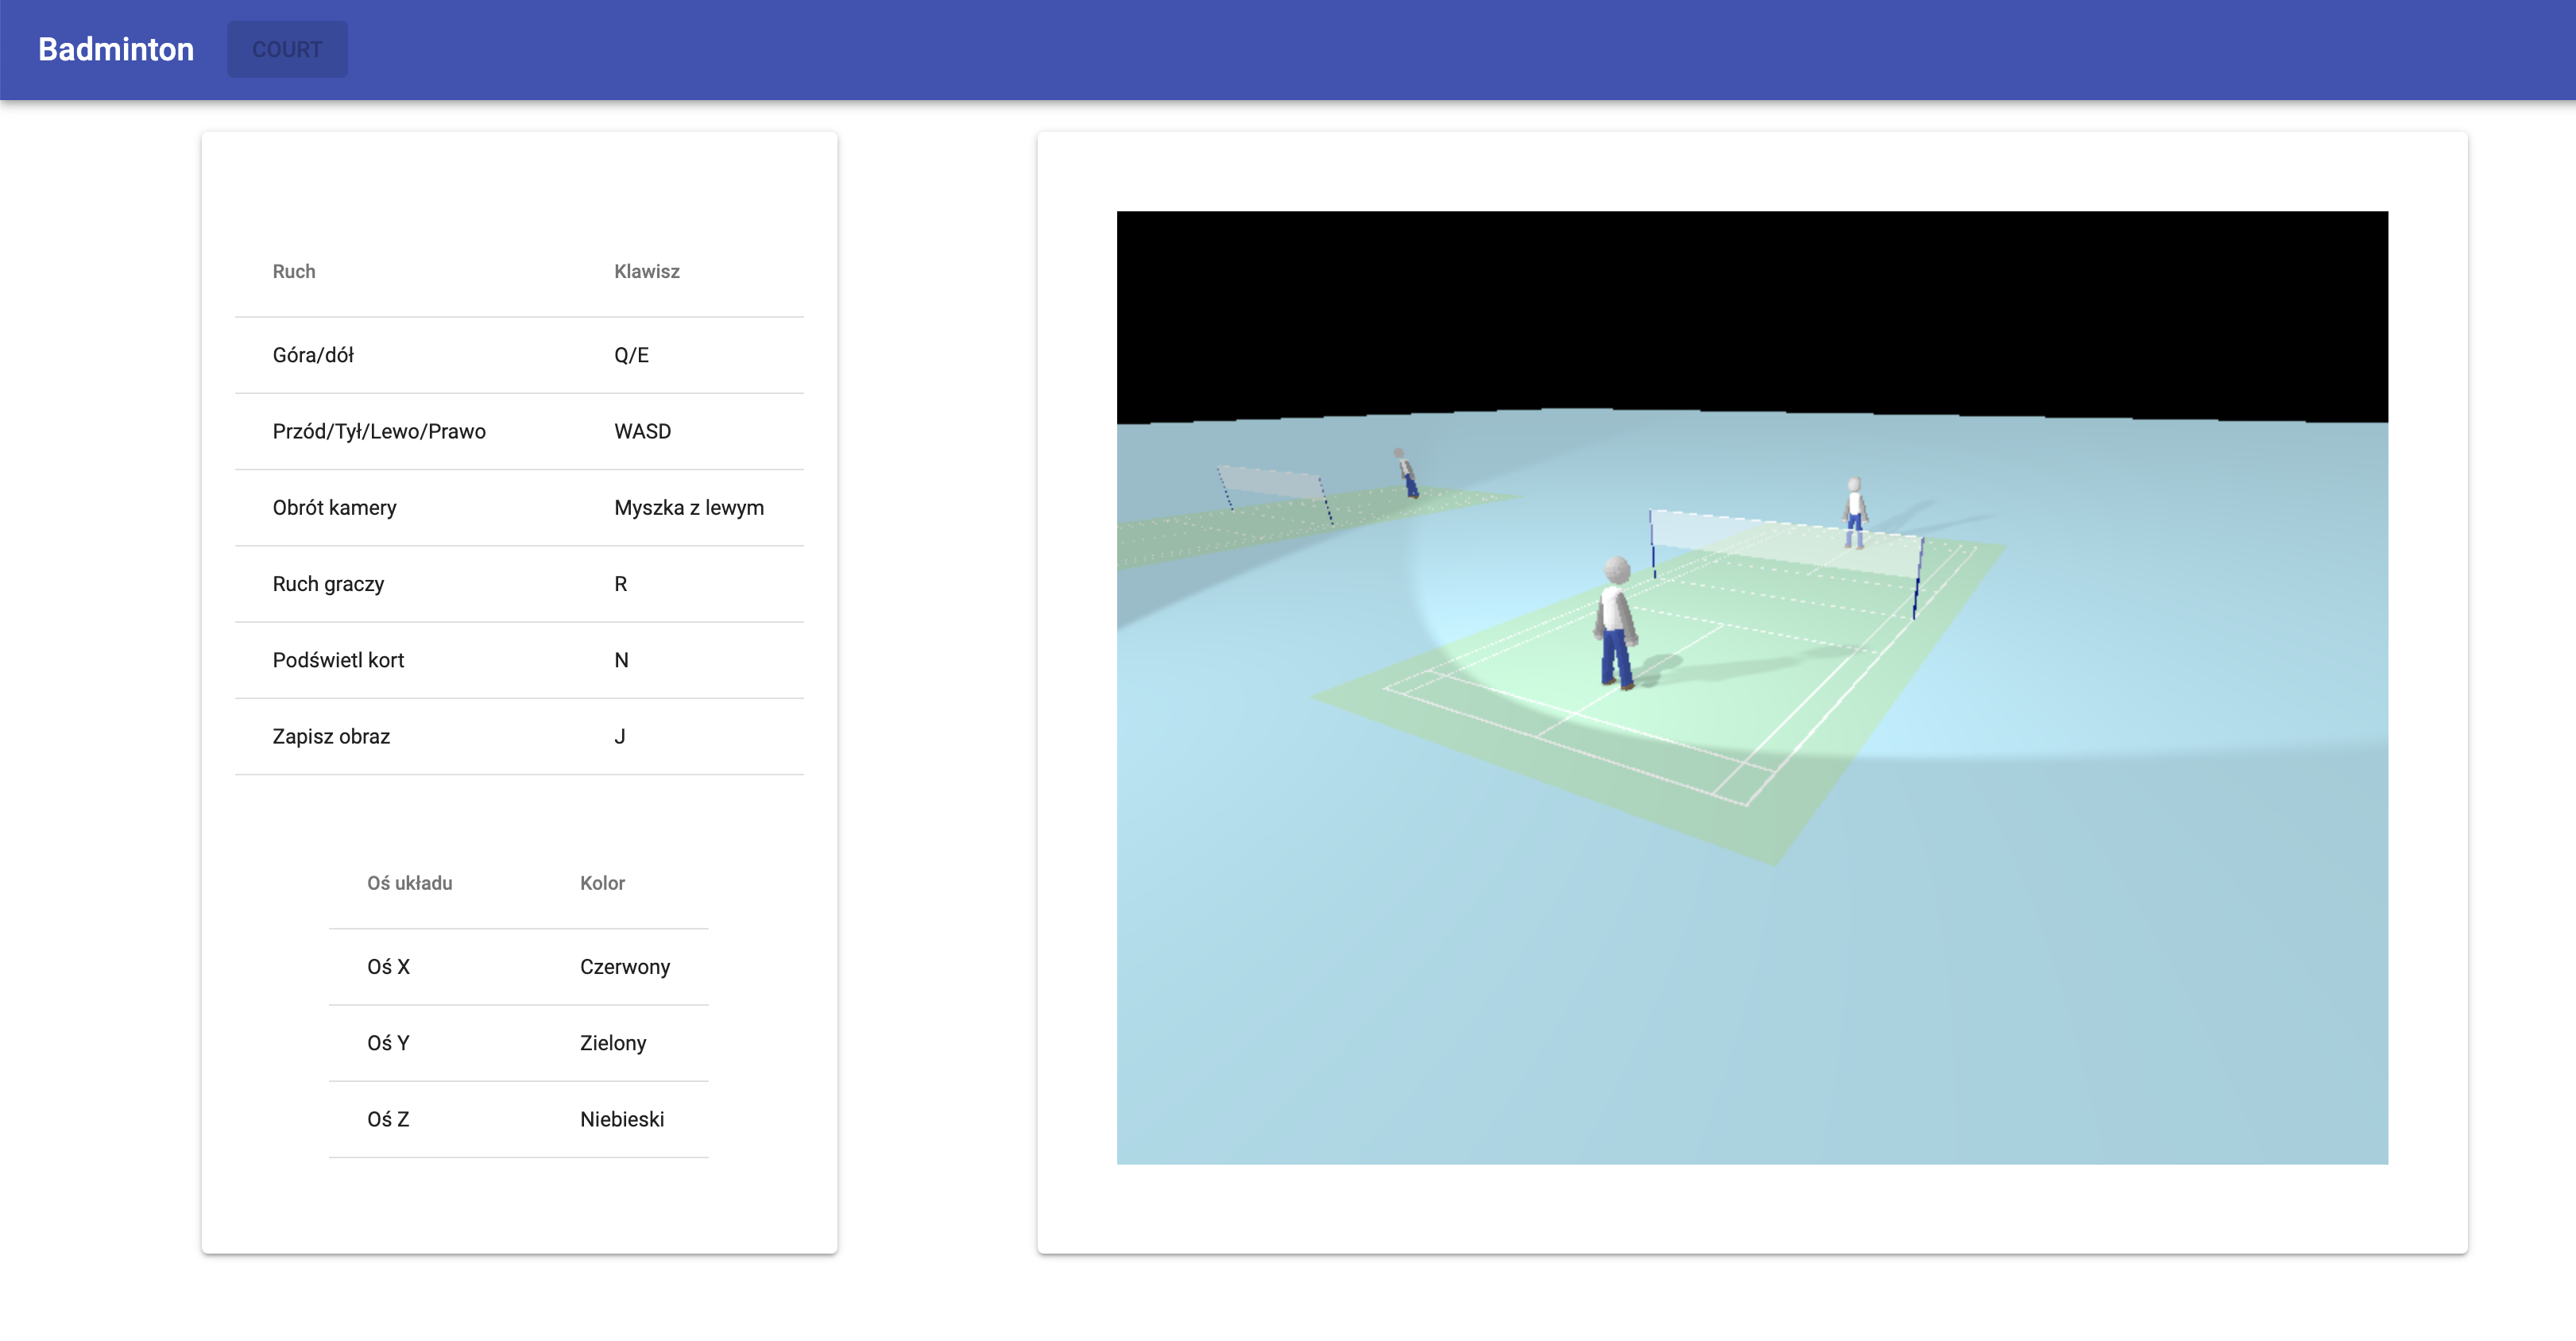
\includegraphics[width=\linewidth]{./generator_1.png}
    \caption{Zrzut ekranu uruchomionego generatora sztucznych danych}
\end{figure}
